\documentclass[a4paper,9pt]{ltjsarticle}
\usepackage{graphicx}
\usepackage{luatexja-fontspec}
\usepackage{caption}
\usepackage{amsmath,amssymb,bm,braket,amsmath,latexsym, mathtools}
\usepackage[english]{babel}
\usepackage{physics}
\usepackage{multicol}
\usepackage{titlesec}
%\usepackage{gnuplot-lua-tikz}
\usepackage[top=20truemm,bottom=20truemm,left=20truemm,right=20truemm]{geometry}
\usepackage{array}
\usepackage{upgreek}
\usepackage{fancyhdr}
\renewcommand{\refname}{}
\usepackage{listings,jvlisting}
\usepackage{tikz}
\usepackage[version=3]{mhchem}
\usetikzlibrary{external}
\tikzexternalize
\lstset{
  basicstyle={\ttfamily},
  identifierstyle={\small},
  commentstyle={\smallitshape},
  keywordstyle={\small\bfseries},
  ndkeywordstyle={\small},
  stringstyle={\small\ttfamily},
  frame={tb},
  breaklines=true,
  columns=[l]{fullflexible},
  numbers=left,
  xrightmargin=0pt,
  xleftmargin=3pt,
  numberstyle={\scriptsize},
  stepnumber=1,
  numbersep=1pt,
  lineskip=-0.5ex
}
\captionsetup[figure]{format=plain, labelformat=simple, labelsep=quad,labelfont=bf,name={Fig.}}
\captionsetup[table]{format=plain, labelformat=simple, labelsep=quad,labelfont=bf}
\parindent = 0pt
%[BoldFont=HGSMinchoE]{MSMincho}[BoldFont=HiraMinProN-W6]{HiraMinPro-W3}
\pagenumbering{gobble}

\begin{document}
\centerline{\Large\bfseries unfolding Color Codeの誤り耐性}
\vspace{10pt}
\section{仮定}{
     符号を用いているとき、エラーはシンドローム測定や誤り訂正中に発生しないと仮定する。もし仮にシンドローム測定中や誤り訂正中にエラーが起きたとするならば、それは次のroundで訂正することとする。このことをわかりやすく、Fig.\ref{figure1}に示した。Fig.\ref{figure1}に示す通り、round 2の操作時に発生するエラーは、round 2-round 3間の論理操作時に発生するエラーと置き換えることができると仮定するということである。そのため、round $t$ではround $t-1$-round $t$間のエラーが訂正できれば良い。
    \begin{figure}[h]
        \centering
        \includegraphics[scale=0.5]{figure/figure1.eps}
        \caption{ }
        \label{figure1}
    \end{figure}

    このようなことを前提として以下ではunfolding Color Codeの誤り耐性、具体的にはColor CodeからSurface Codeへの変換(Fig.\ref{figure1}でいうとシンドローム測定)の際に発生したエラーがその変換後に検出できるのかということを確認していく。\\
}
\section{エラー検出}{
     まず、Stabilizer Codeではどのようにしてエラーを検出しているのかということを確認する。ここで、round $t$でのphysical qubitsの状態は$\ket{\psi}^t$と表され、round $t$ではエラーは発生していないとする。また、stabilizer groupを$\mathcal{S}$とする。round $t$でスタビライザー $s_j\in \mathcal{S}$についてシンドローム測定を行うと、
    \begin{align}
        s_j\ket{\psi}^t=m^{t}_j\ket{\psi}^t
    \end{align}
    が成り立つ。ただし、$m^{t}_j$はround $t$での$s_j$のシンドローム値を表す。スタビライザー符号ではよくスタビライザー状態を$m_j=1$として定義するが、実際にエラーを検出するときは$m=-1$のときをスタビライザー状態としても同じであり、このときは$m_j=1$のときにエラーが発生していることになる。次に、round $t$-round $t+1$間で論理操作をし、round $t+1$で$s_j\in \mathcal{S}$についてシンドローム測定を行うと、
    \begin{align}
        s_j\ket{\psi}^{t+1}=m^{t+1}_j\ket{\psi}^{t+1}
    \end{align}
    が成り立つ。このとき、round $t$-round $t+1$間で$s_j$によって検出されるようなエラーが発生していたら、$m^{t+1}$と$m^{t}_j$の符号は逆、すなわち$m^{t+1}m^{t}_j=-1$、round $t$-round $t+1$間で$s_j$によって検出されるようなエラーが発生していなければ、$m^{t+1}_{j}$と$m^{t}_j$の符号は同じ、すなわち$m^{t+1}m^{t}_j=1$となる。このようなことから、round $t$-round $t+1$でのエラー検出はすべてのスタビライザーに対して、$m^{t+1}_{j}m^{t}_j$を考えれば良く、$m^{t+1}_{j}m^{t}_j=-1$のとき、エラーが起こったとする。
}
\clearpage
\section{unfolding操作でのエラー検出}{
    Color Codeのunfolding操作はFig.\ref{figure2}のようにして行われる(詳細は前回の資料unfolding\_color\_code.pdfを参照)。

    \begin{figure}[h]
        \centering
        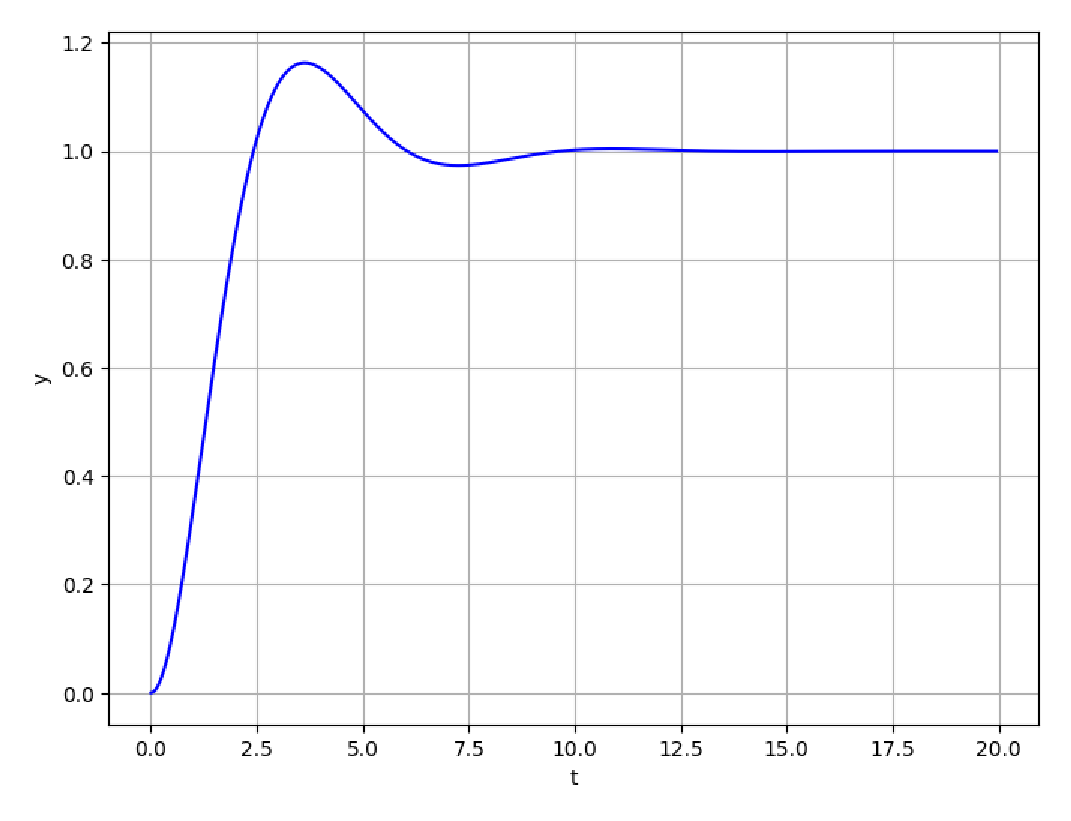
\includegraphics[scale=0.2]{figure/figure2.eps}
        \caption{ }
        \label{figure2}
    \end{figure}

    ここでの議論はround $t$でFig.\ref{figure2}の左の状態、round $t+1$でFig.\ref{figure2}の右の状態であるとする。また、符号距離は一般の$d$のときについて議論する。\\
     まずもともとColor Codeだった領域でunfolding操作中に発生したXエラーに注目する(Fig.\ref{figure3})。

    \begin{figure}[h]
        \centering
        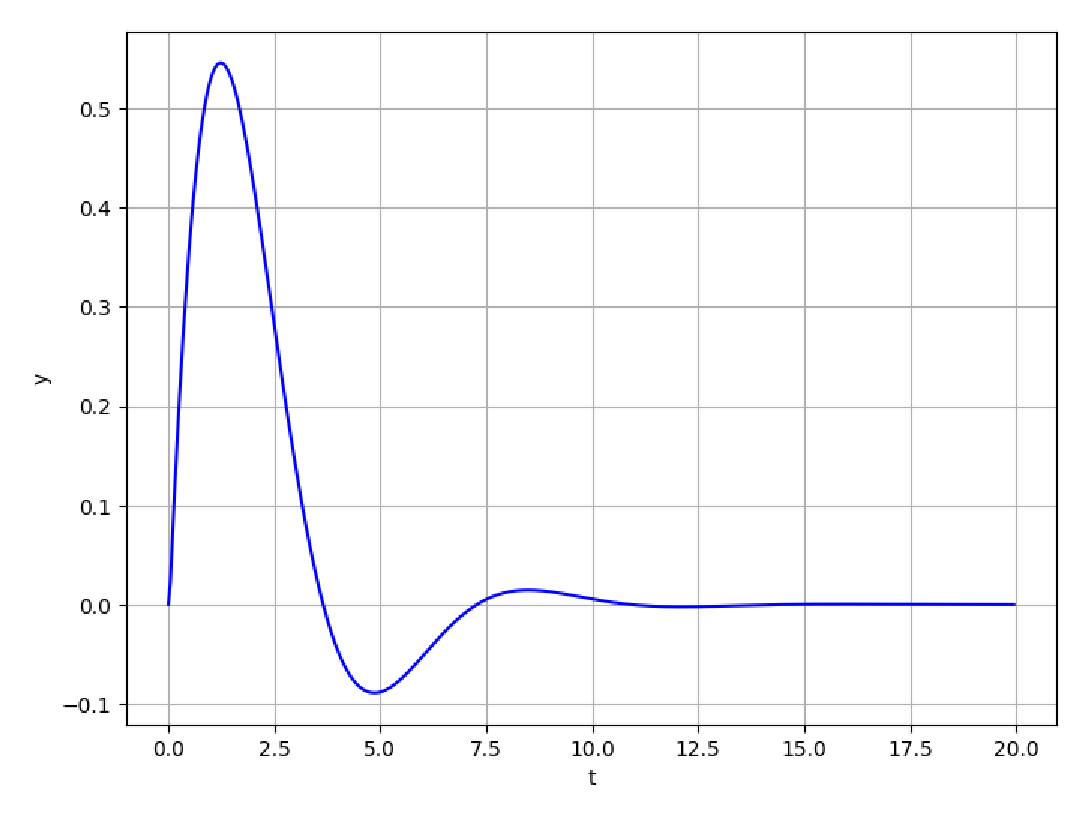
\includegraphics[scale=0.2]{figure/figure3.eps}
        \vspace{-20pt}\caption{ }
        \label{figure3}
    \end{figure}

    Fig.\ref{figure3}で見えているスタビライザーについて、Color Codeのblue face Z スタビライザー、red face Z スタビライザーをそれぞれ$s^\text{b}_\text{CC}, s^\text{r}_\text{CC}$、Surface CodeのZ スタビライザーでもともとblue face だった部分、red face だった部分を$s^\text{b}_\text{SC}, s^\text{r}_\text{SC}$と表す。また、$s^i_j$のシンドローム値を$m^i_j$とする。このとき、Fig.\ref{figure3}に示されているX エラーというのは$s^\text{b}_\text{SC}, s^\text{r}_\text{SC}$のシンドローム値を反転させる。つまり、$m^\text{b}_\text{SC}m^\text{b}_\text{CC}=-1,\ m^\text{r}_\text{SC}m^\text{r}_\text{CC}=-1$となり、発生したX エラーを検出できる。すなわち、Fig.\ref{figure4}のように、Surface Code上ではanyon modelを用いて粒子mが発生したのと同じである。あとはSurface Codeと同じように誤り訂正すれば良い。Boudary部分についても同じような議論ができる。また、もともとColor Codeではなかった部分のXエラーについても、最初はZ方向に初期化されていることから、操作前のシンドローム値は初期化したときの1つの正六角形状の6つのqubitの測定値の積と、その場所のSurface Codeのシンドローム値を比べることによってX エラーを検出できる。Bundary に2-weightスタビライザーが存在する場合があるが、それも同じようにできる。

    \begin{figure}[h]
        \centering
        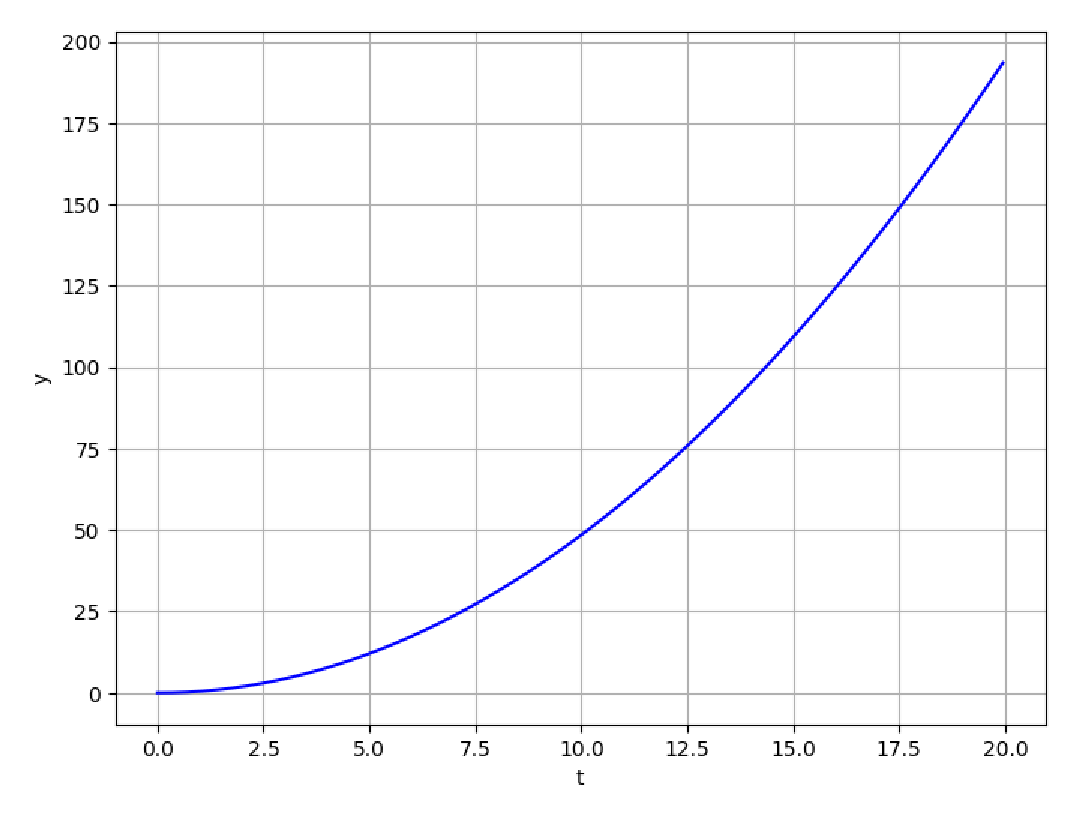
\includegraphics[scale=0.18]{figure/figure4.eps}
        \vspace{-20pt}\caption{ }
        \label{figure4}
    \end{figure}

     次にもともとColor Codeだった領域でunfolding操作中に発生したZエラーに注目する(Fig.\ref{figure5})。

    \begin{figure}[h]
        \centering
        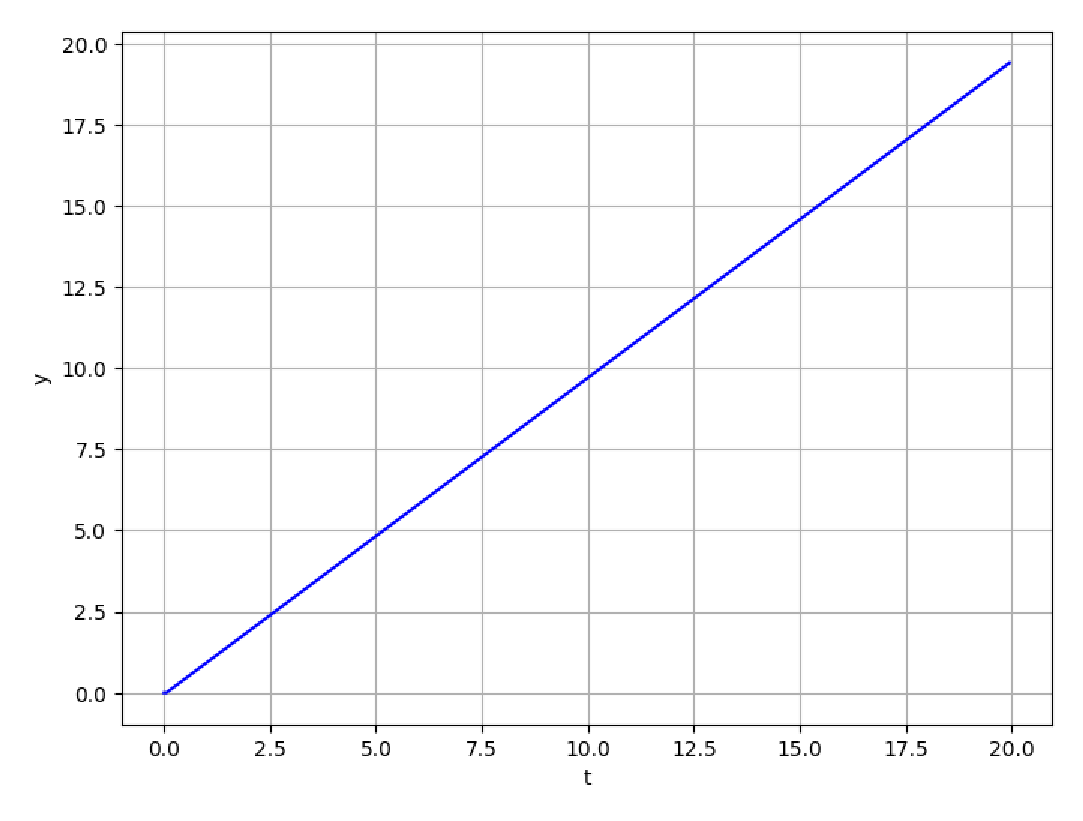
\includegraphics[scale=0.18]{figure/figure5.eps}
        \vspace{-20pt}\caption{ }
        \label{figure5}
    \end{figure}
    unfolding操作の2-weight X スタビライザーはred faceのZスタビライザーと反可換であるため、いくつかの2-weight X スタビライザーはundeterministicである。しかし、エラーが存在しなければ、1つのblue face(red face)上の3つの2-weight X スタビライザーの積はdeterminisicでColor Codeのときの6-weight X スタビライザーのシンドローム値と同じでなければならない。すなわち、Fig.\ref{figure5}のZ エラーは検出できる。また、anyon modelで表すとFig.\ref{figure6}となる。


    \begin{figure}[h]
        \centering
        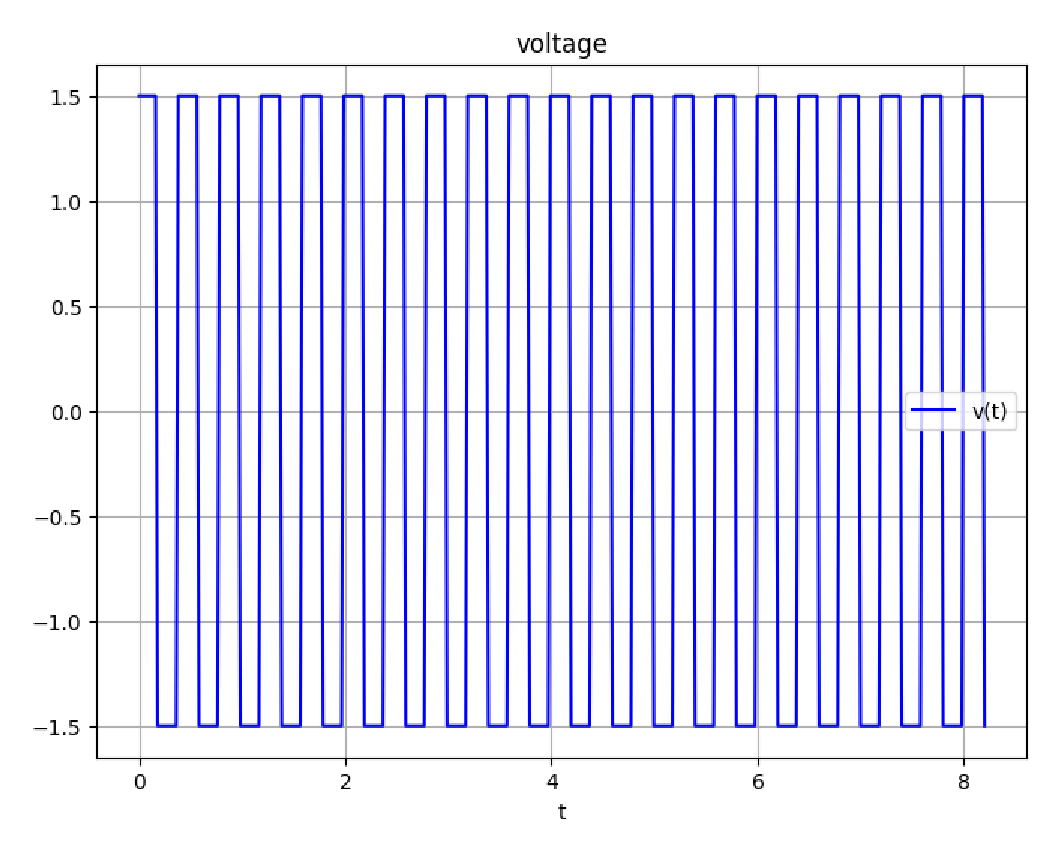
\includegraphics[scale=0.18]{figure/figure6.eps}
        \vspace{-20pt}\caption{ }
        \label{figure6}
    \end{figure}

    エラーの位置がわかるので、これをSurface Codeの描像にmappingするとFig. \ref{figure7}のようになる。また、$\ket{0}$に初期化する領域にはZ エラーが起きない(?)ので考える必要は無い。あとはSurface Codeと同じように誤り訂正すれば良い。

    \begin{figure}[h]
        \centering
        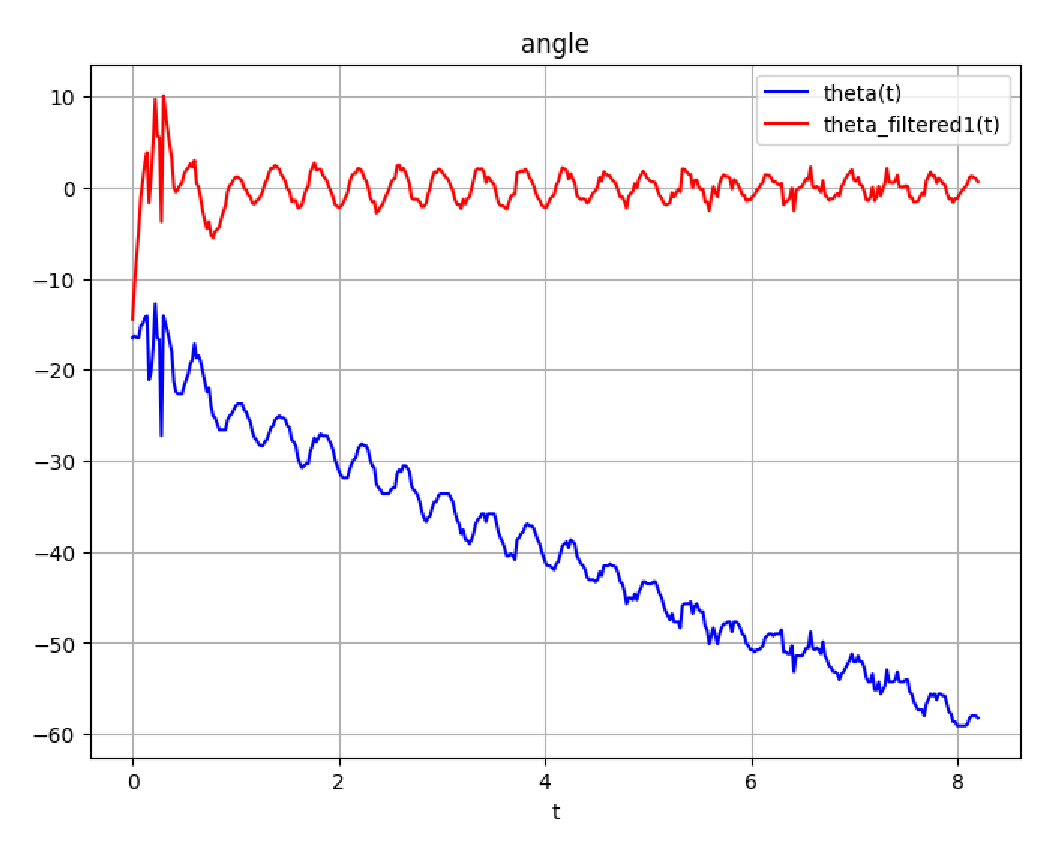
\includegraphics[scale=0.18]{figure/figure7.eps}
        \vspace{-20pt}\caption{ }
        \label{figure7}
    \end{figure}
}
\clearpage

\section{mapping}{
    実際にSurface Codeの描像へのmappingがうまくできるか検証してみる。\\
     まず、X エラー検出は素直にできる(Fig.\ref{figure8})。ここで、黄色のチェインはX エラーを表す。

    \begin{figure}[h]
        \centering
        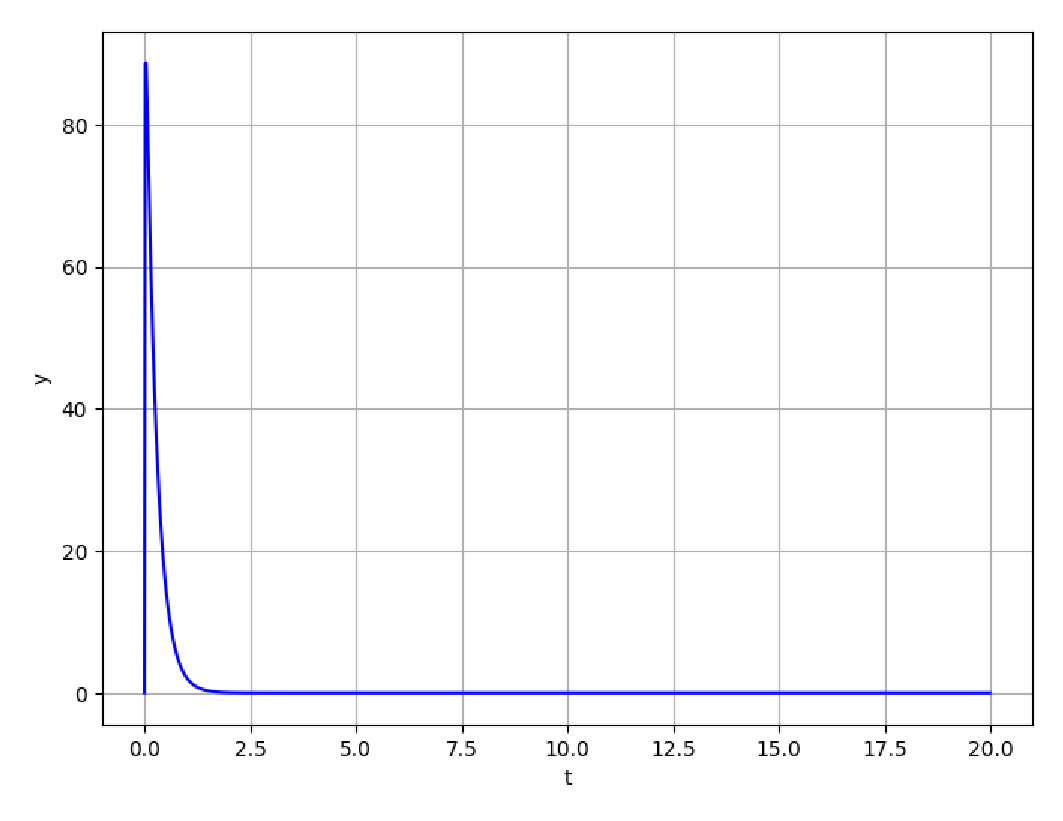
\includegraphics[scale=0.18]{figure/figure8.eps}
        \vspace{10pt}\caption{ }
        \label{figure8}
    \end{figure}

    次に、Z エラーの検出だが、これは少し工夫が必要である。Fig. \ref{figure9}、Fig. \ref{figure10}に2パターン示す。ここで、黄色のチェインはZ エラーを表す。行っていることは、Surface Codeの描像のanyon modelで表せるまで、Fig. \ref{figure7}の形を作って変換しているだけである。本当は右上半分にはZ エラーは存在しない(?)が、存在しないほうが簡単なのであまり気にしなくても良い。

    \begin{figure}[h]
        \centering
        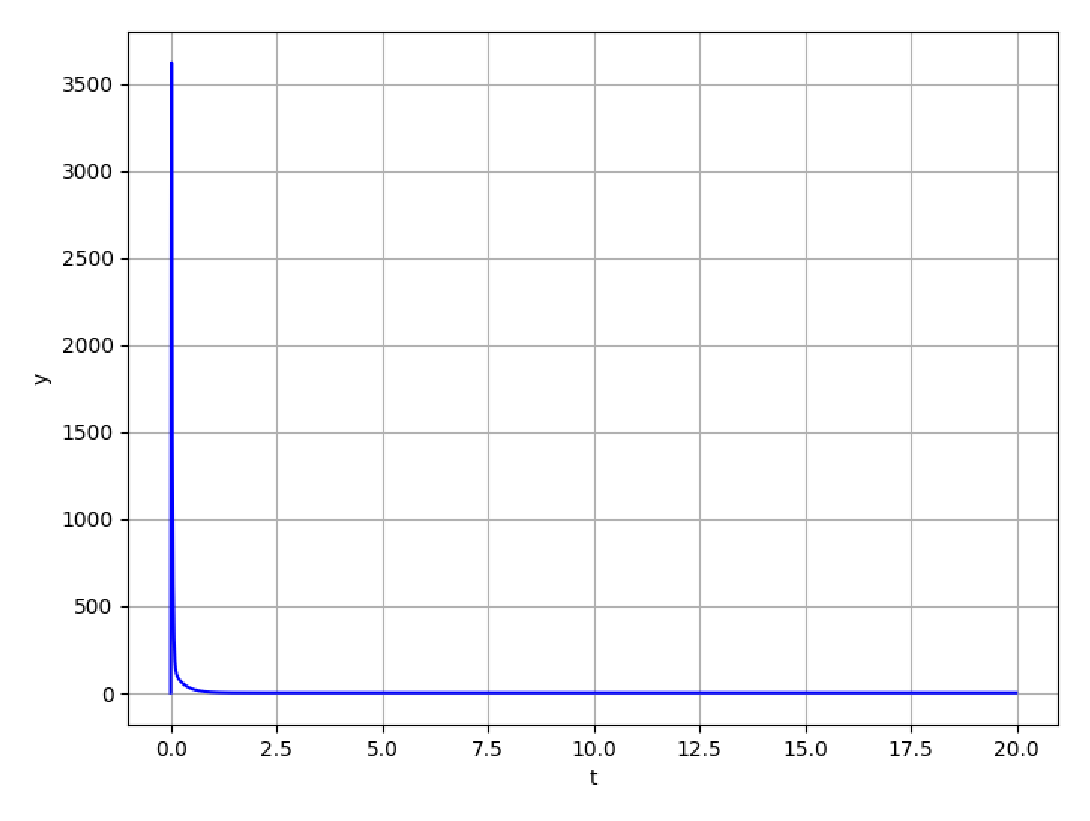
\includegraphics[scale=0.20]{figure/figure9.eps}
        \vspace{10pt}\caption{ }
        \label{figure9}
    \end{figure}
    \begin{figure}[h]
        \centering
        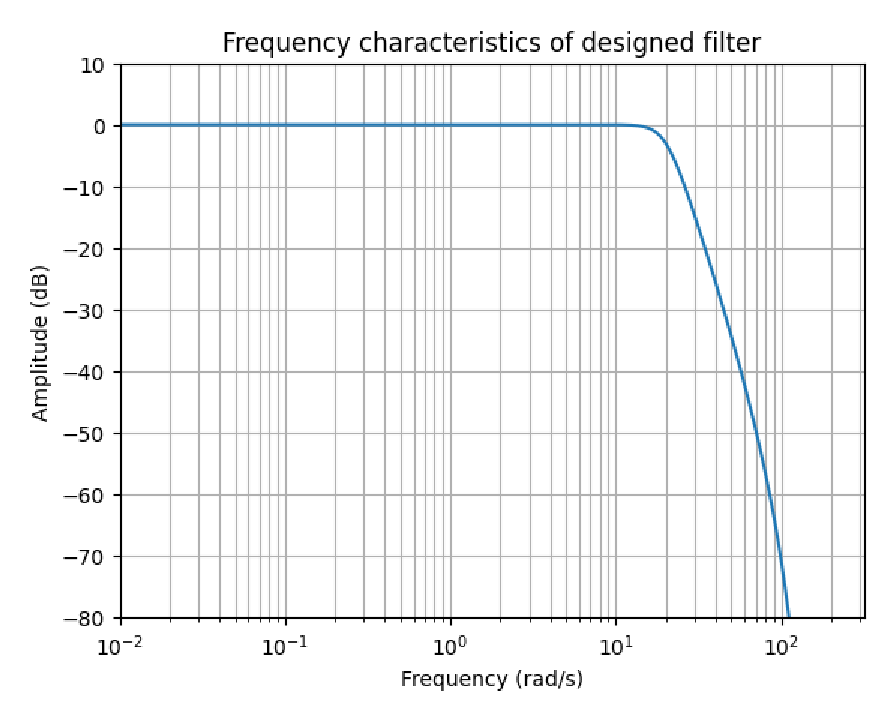
\includegraphics[scale=0.20]{figure/figure10.eps}
        \vspace{10pt}\caption{ }
        \label{figure10}
    \end{figure}

    あらゆるパターンをこのように変換できる(?)。
}

\end{document}